\documentclass[a4paper,12pt]{article}

\usepackage{graphics}
\usepackage{graphicx}
\usepackage{float}
\usepackage{hyperref}

\hypersetup{ colorlinks=true, linkcolor=blue, filecolor=magenta, urlcolor=cyan }

\begin{document}
	\begin{titlepage}
		\title{Interim Planning and Investigation Report}
		\date{\today}
		\author{Ibraheem Ganiyu}
	\end{titlepage}
	\maketitle
	
	\pagenumbering{roman}
	\tableofcontents
	\newpage
	\listoffigures
	\listoftables
	\newpage
	\pagenumbering{arabic}
	
	\section{Project Scope}
		\subsection{Aims and Objectives}
		The project aims to apply complex machine learning models to the prediction of drugs that can penetrate through the blood brain barrier. \\
		Extensive background study would be conducted on the fields of drug design and discovery in the context of the central nervous system (CNS) and in the penetration of the blood brain barrier (BBB). 
		\subsection{Stakeholders and their Interests}
		The primary stakeholder is my project supervisor Aidan Delaney. The interest would be in a system that can deliver a very high prediction accuracy as systems in recent research papers.
		\subsection{Methods of Communication}
		The main method of communication would be through weekly meetings, where what has been done so far would be reviewed and tasks also set for the following week. Communications would also take place via emails and impromptu meetings to supplement the weekly meetings.
		\subsection{Project Infrastructure}
		The end result would be a software system available via the internet that can be part of a drug discovery pipeline in the design of drugs for treating diseases associated with the brain. A typical drug pipeline consist of the target identification, hit \& target identification, pre-clinical, clinical trials and then regulatory approval stage. The system produced by the project can be deployed in the hit \& target identification stage of the pipeline as it aims to help identify the drugs which have the highest probabilities of penetrating the BBB. 
		\subsection{Installation Standards and Procedures}
		To circumvent the problem of cross platform software development. The software application will be packed in a Docker container and deployed on the host machine.
		\subsection{Quality Checks}
		To measure the quality of the delivered software. The following conditions must be met
		\begin{itemize}
			\item The application should compile successfully 
			\item The application should listen for connections on the web and produce a thin web client as a default response
			\item The application should accept the SMILE molecular format via a REST API and return the probability of the posted SMILE passing through the BBB to the client
		\end{itemize}
	
	
	\section{Project Specification}
	The following are the main stages of the project. Each stage represents a significant step in the forming of the main product
		\subsection{Deliverables}
			\begin{itemize}
				\item \underline{Data Cleaning}: The original data is a list of SMILES, it has to be processed and transformed for use with our program. To reduce the start-up time of our software, a significant proportion of the data would be processed and saved to disk for use later.
				\item \underline{Classifier Training}: Based on the literature reading, a select group of classifiers would be trained with our data. An Extension would be to train the classifier on different clusters to improve the overall training time.
				\item \underline{Ensemble Learning}: All the trained classifiers would be combined into one big classifier that uses a voting mechanism to predict results.
				\item \underline{Deployment}: The ensemble classifier would be utilised in a web server that would serve as the middle-man between the classifier and the client. The server would be deployed in a docker container for portability and communicate via HTTP.
				\item \underline{Testing and Quality Assurance}: The overall program would be run across a comprehensive test suite to ensure all set quality assurance criteria are met.
			\end{itemize}
			% Gantt chart developed using https://app.ganttpro.com/#!/app/home. Logon {email:ruhapif@dr69.site}
			\begin{figure}[H]
				\centering
				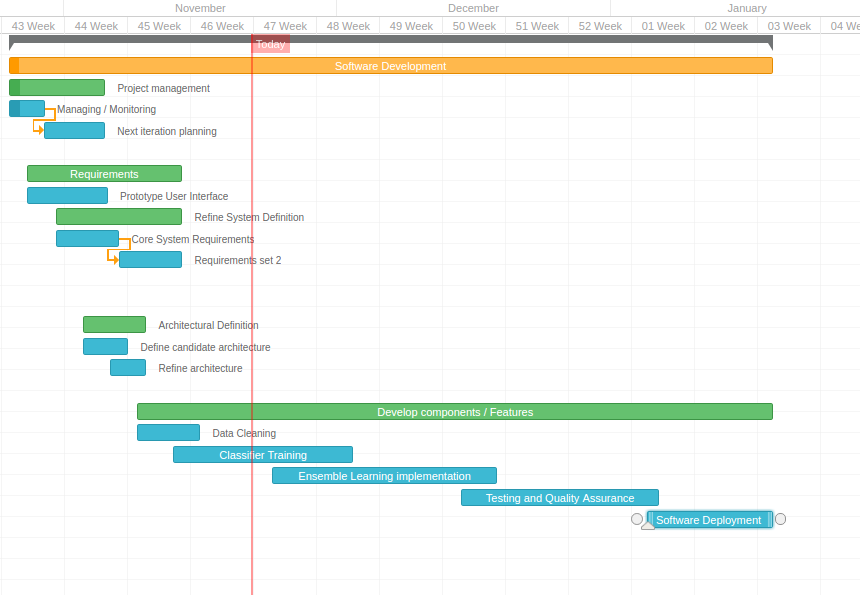
\includegraphics[width=\textwidth,scale=1]{images/bbb_gantt}
				\caption{Project Gantt Chart}
				\label{fig:bbb_gantt}
			\end{figure}
		\subsection{Risk Analysis}
		A further risk assessment has been carried out on the project and the conclusions recorded in the table below
		\begin{table}[ht]
			\caption{Risk Assessment Chart}
			\centering
			\begin{tabular}{c|c|c|c}
				\hline \hline
				Vulnerability & Probability & Magnitude & Impact Rating \\
				\hline
				Broken SMILES in Data & Possible & Moderate & 50 \\
				Inaccurate Predictions & Probable & Critical & 90 \\
				Compatible issues in ensemble learning & Highly Unlikely & Major & 60 \\
				Cluster failure during training & Possible & Minor & 25 \\
				Server failure post-production & Possible & Critical & 75
			\end{tabular}
		\end{table}
	
	
	\section{Product Description}
	The product is codenamed "The endurance" and it identifies itself as a drug discovery tool that can be integrated into a drug discovery pipeline.
		\subsection{Purpose}
		The primary purpose of the tool is to predict the probability of a molecule passing through the blood brain barrier. It also serves the following functions
			\begin{itemize}
				\item An experimentation platform for analysing the effects of different machine learning classifiers on the BBB prediction
				\item A platform for the analysis of the BBB penetration of a large set of molecules.
			\end{itemize}
		\subsection{Product Derivation}
		The product is highly inspired by \href{http://www.atomwise.com/}{Atomwise} , a company applying artificial intelligence techniques to the creation of better drugs and \href{http://b3pp.lasige.di.fc.ul.pt/about.html}{B3PP}, an already existing on-line platform for the prediction of BBB penetration of drugs
		\subsection{Product Composition and Form}
		The product is composed of the 3 parts
			\begin{itemize}
				\item The Web Client \\ The web client acts as a tool that accepts molecular SMILES either through a line entry system or via a bulk upload, it then interfaces with the server and returns the result to the client
				\item Web Server \\ The Server acts as the middle man between the web client and the prediction engine, conveying messages between the client and the prediction engine and also coordinates the life cycle of the engine.
				\item Prediction Engine \\ The engine represents an ensemble classifier. The ensemble classifier consists of different classifiers trained on numerous clusters consolidated into a single classifier, and it uses a voting mechanism to determine the best result for each prediction task.
			\end{itemize}
		\subsection{Relevant Standards}
		The web client adheres to the W3C standards for web applications and for web services.
		%\subsection{Development Methodology}
		
	
	\section{Literature Review}
	Historically, parts of trees have always been used to cure or alleviate symptoms of illness and over time the individual molecules in these herbal medicines were recognized for their effects and produced synthetically. Modern drug discovery is a very expensive and time consuming process; It is usually broken down into numerous stages with the most expensive stage being Clinical trials. A potential drug candidate is usually screened against a target protein to test its effectiveness and the screening can either be virtual (Virtual Screening) or through a method known as High Throughput Screening (HTS) - a method of experimentation involving the use of robots and control software to conduct millions of scientific tests. These HTS machines can also be credited with the exponential growth in chemical data  \cite{Dougetal2008}
	\\
	This section will explain explain in detail the drug discovery and design process and the discovery process in Central Nervous System (CNS) drug design and then illustrate how Machine Learning fits into this picture and how it can be applied to the Blood Brain Barrier (BBB) prediction problem
		\subsection{Drug Discovery and Design}
		According to Dr A.N Boa \cite{hull2016}, the different stages of drug discovery are
			\begin{itemize}
				\item Programme Target Selection (Choosing the disease to work on)
				\item Identification and Validation of the drug target
				\item Assay Development
				\item Identification of a Lead Compound
				\item Lead Optimisation
				\item Identification of a drug candidate 
				\item Clinical Trials 
				\item Release of the drug 
				\item Follow-up Monitoring
			\end{itemize}
		Majority of the targets for the drugs we consume are usually proteins e.g enzymes, receptors and nucleic acids and the structure of the target is confirmed through a virtual screening method known as \textit{molecular docking}; it can be used to predict how the drug will bind to its target protein though various search/optimisation algorithms \cite{Jurgen2004}.
		Another Virtual Screening technique usually used is \textit{Quantitative Structure-Activity Relationships} (QSAR), here the underlying idea is that molecules with similar structures behave in the same way, as a result, the activity of a protein against a certain group of compounds is recorded and a QSAR model is the constructed from there and used to determine whether a given compound will bind to the target, thus screening the virtual compound library for drugs of interest.
		\subsection{CNS Drug Design and the Blood Brain Barrier}
		CNS Drugs aiming to pass through the Blood Brain Barrier often need to possess certain physical-chemical properties; some of which are Hydrogen bonding, ionization properties, molecular flexibility etc. \cite{Hassanetal2005}. The epithelial cells form an interface between the blood and the brain and these are commonly referred to as the Blood Brain Barrier. This interface occurs in other places within the body but what makes the BBB epithelial cells different are the tight junctions they form which makes it harder for drugs to pass through. Hassan and George (2005) further claim in their article that the majority of BBB penetration is through passive diffusion through the cellular membrane.
			\subsubsection{ADME Properties of CNS Drugs}
			For a CNS drug to be therapeutically effective, it must be easily disposed asides from having a high degree of potency. The ADME properties of a drug refers to its ability to be easily absorbed, distributed, metabolised and excreted. Some properties of CNS drugs affect their ADME properties, some of which are \cite{Hassanetal2005}:
				\begin{itemize}
					\item \underline{Solubility}: A drug must be very soluble in the blood and still be in high enough concentration at its target, in this case, the Blood Brain Barrier, so that it can easily be absorbed.
					\item \underline{Amount of Protein Binding}: Majority of CNS drugs tend to have high binding property towards proteins - this results in the drug being metabolised easily.
					\item \underline{Partition Coefficient (LogP)}: This is sometimes referred to as the \textit{lipophilicity} of the compound and has served as one of the most important factors in drug design. Higher lipophilicity results in drugs with higher metabolic turnover but lower solubility and absorption \cite{Hassanetal2005}. 
				\end{itemize}	
		\subsection{Machine Learning in Drug Discovery and Design}
		With the recent explosion in chemical data available, it is possible to combine them with machine learning techniques to create models of molecules that have a strong binding affinity to their target proteins. According to Antonio (2015) \cite{Antonio2015}, Virtual screening techniques can either be Structure-Based or Ligand-Based. Structural screening used the idea of molecular docking as described earlier whilst Ligand-Based screening uses the idea that similar molecules exhibit similar properties e.g QSAR. 
		\\
		With Ligand-Based Virtual Screening being the core focus of this paper, we can further classify them into either similarity searching or compound classification \cite{Antonio2015}. Antonio (2015) \cite{Antonio2015} further highlights that the following are the most popular and successful techniques for Ligand-Based Virtual Screening:
			\begin{itemize}
				\item Support Vector Machines
				\item Decision Trees
				\item Random Forests (An Ensemble of Decision Trees)
				\item Naive Bayesian Classifiers
				\item k-Nearest neighbours
				\item Artificial Neural Networks
			\end{itemize} 
	
	\section{Conclusion} 
	This projects aims to produce a program that can predict the probability of a drug passing through the Blood Brain Barrier; such a program would prove useful in a drug development pipeline especially in CNS drug discovery.
	
	\newpage
	
	\section{Annotated Bibliography}
		\subsection{Big data: The future of biocuration}
		It highlights the benefits big data has in the scientific space and it also shows the different kinds of scientific data and how they can be used for experimentation; It also shows the different open data sources available for public use. It benefits my research as it provides a starting point for collecting data for use in training and testing the proposed system.
		\subsection{Introduction to Drug Discovery}
		This online article gives a brief overview of the entire process of drug discovery and describes in detail each process involved. Although not as detailed, It would prove useful for my research by providing a starting point to begin analysing other researches in the field.
		\subsection{Chemoinformatics: Concepts, Methods and Tools for Drug Discovery}
		A very technical book on Computational Chemistry, it explains in detail every aspect of chemoinformatics and how it relates to the drug discovery process. It would serve as a valuable resource for providing the technical know-how on certain aspects of implementing the proposed systems especially with respect to processing chemical data.
		\subsection{Medicinal Chemical Properties of Successful Central Nervous System Drugs}
		An article detailing information about Drug Development for the Central Nervous System, it also provides information about Drug Discovery but in the context of the Blood Brain Barrier. It provides ways on how to approach the prediction problem by highlighting the desired traits of CNS drugs.
		\subsection{Machine Learning approaches in Drug Discovery: methods and applications}
		Being a very important article for my research, it highlights the different ways I can apply my machine learning models to the context of drug discovery. Coupled with the article on \textit{Medicinal Chemical Properties of Successful Central Nervous System Drugs}, they all provide a way to apply machine learning techniques for the Blood Brain Barrier Prediction
	
\newpage
\bibliographystyle{plain}
\bibliography{interim_report}

\end{document}